%% outline-sample.tex
%% Copyright 1991 Peter Halvorson
%% Updates for LaTeX2e copyright 2002 Seth Flaxman
%% Updated for LPPL 1.3c or later by Clea F. Rees (for Seth Flaxman), 2008/10/06.
%
% This work may be distributed and/or modified under the
% conditions of the LaTeX Project Public License, either version 1.3
% of this license or (at your option) any later version.
% The latest version of this license is in
%   http://www.latex-project.org/lppl.txt
% and version 1.3 or later is part of all distributions of LaTeX
% version 2005/12/01 or later.
%
% This work has the LPPL maintenance status `unmaintained'.
%
% This work consists of the files outline.sty and outline-sample.tex.
% Save file as: outline-sample.tex

\documentclass{report}
\usepackage{outlines}
\usepackage{graphicx}
\usepackage{caption}
\usepackage{subcaption}

% [outline] includes new outline environment. I. A. 1. a. (1) (a)
% use \begin{outline} \item ... \end{outline}
		% set second level to enumerate style
% \renewcommand{outlineii}{enumerate}

\pagestyle{empty}


\begin{document}

\noindent \textbf{\Large The Effect of Solid Objects on the \\ Electrostatic Potential} \\

\hrule
\vspace{2cm}

\begin{outline}[enumerate]
\0
  \0 \noindent{\large \bf Speakers}
  
  \1 \textbf{Margarida} \\
  	 Analytical solution \\
  	
  \1 {\bf John} \\
  	 Numerical Methods \\
  	
  \1 {\bf Viktor} \\
  	 Program Structure \\
  	
  \1 {\bf David} \\
  	 Algorithm analysis \\
  	
  \1 {\bf Tristan} \\
  	 Adaptive meshing \\
  	
  \1 {\bf Neil} \\
  	 Analysis \\ \\
  \0 {\large \bf Systems Considered} \\

\end{outline}


\begin{figure}[h!]
\centering
\begin{minipage}{.5\textwidth}
  \centering
  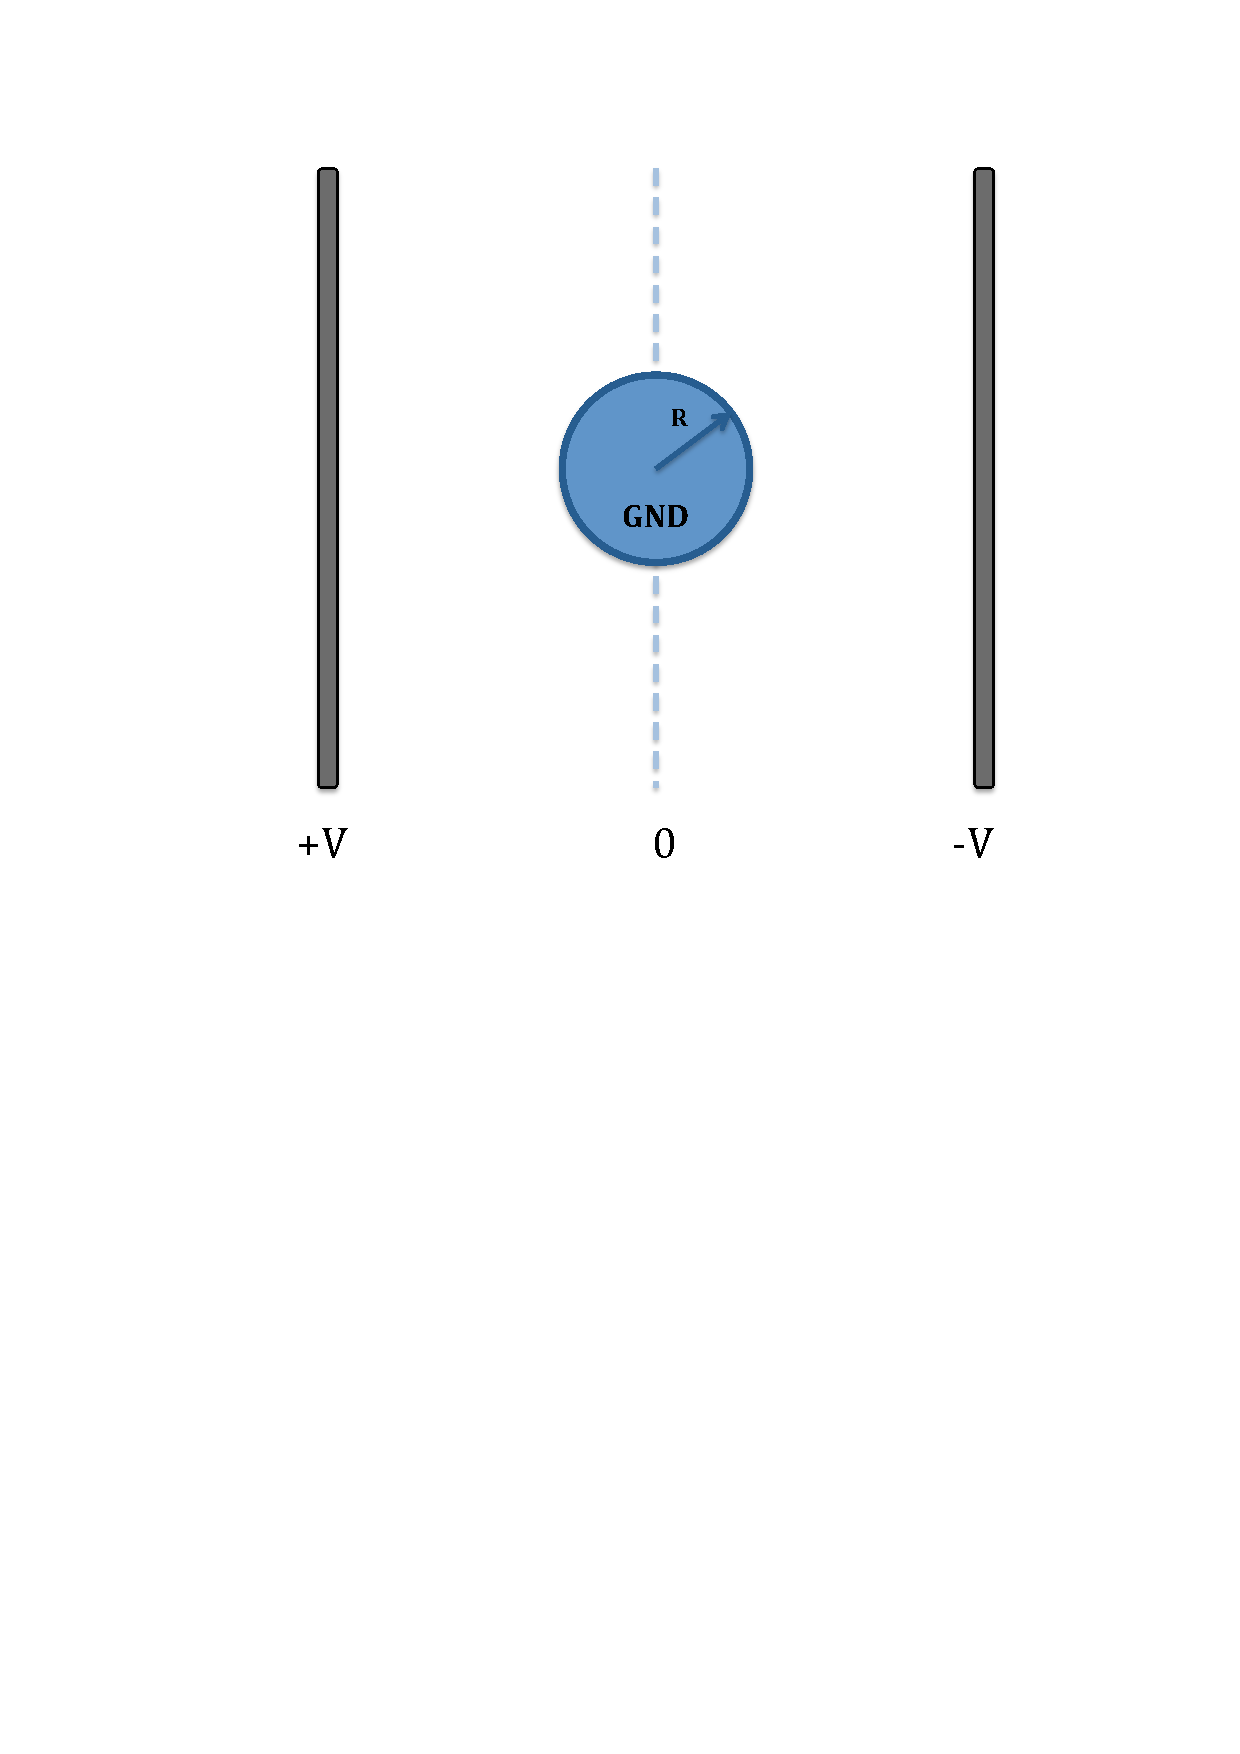
\includegraphics[width=.5\linewidth]{GPdiagramA}
  \captionof{figure}{System A}
  \label{fig:test1}
\end{minipage}%
\begin{minipage}{.5\textwidth}
  \centering
  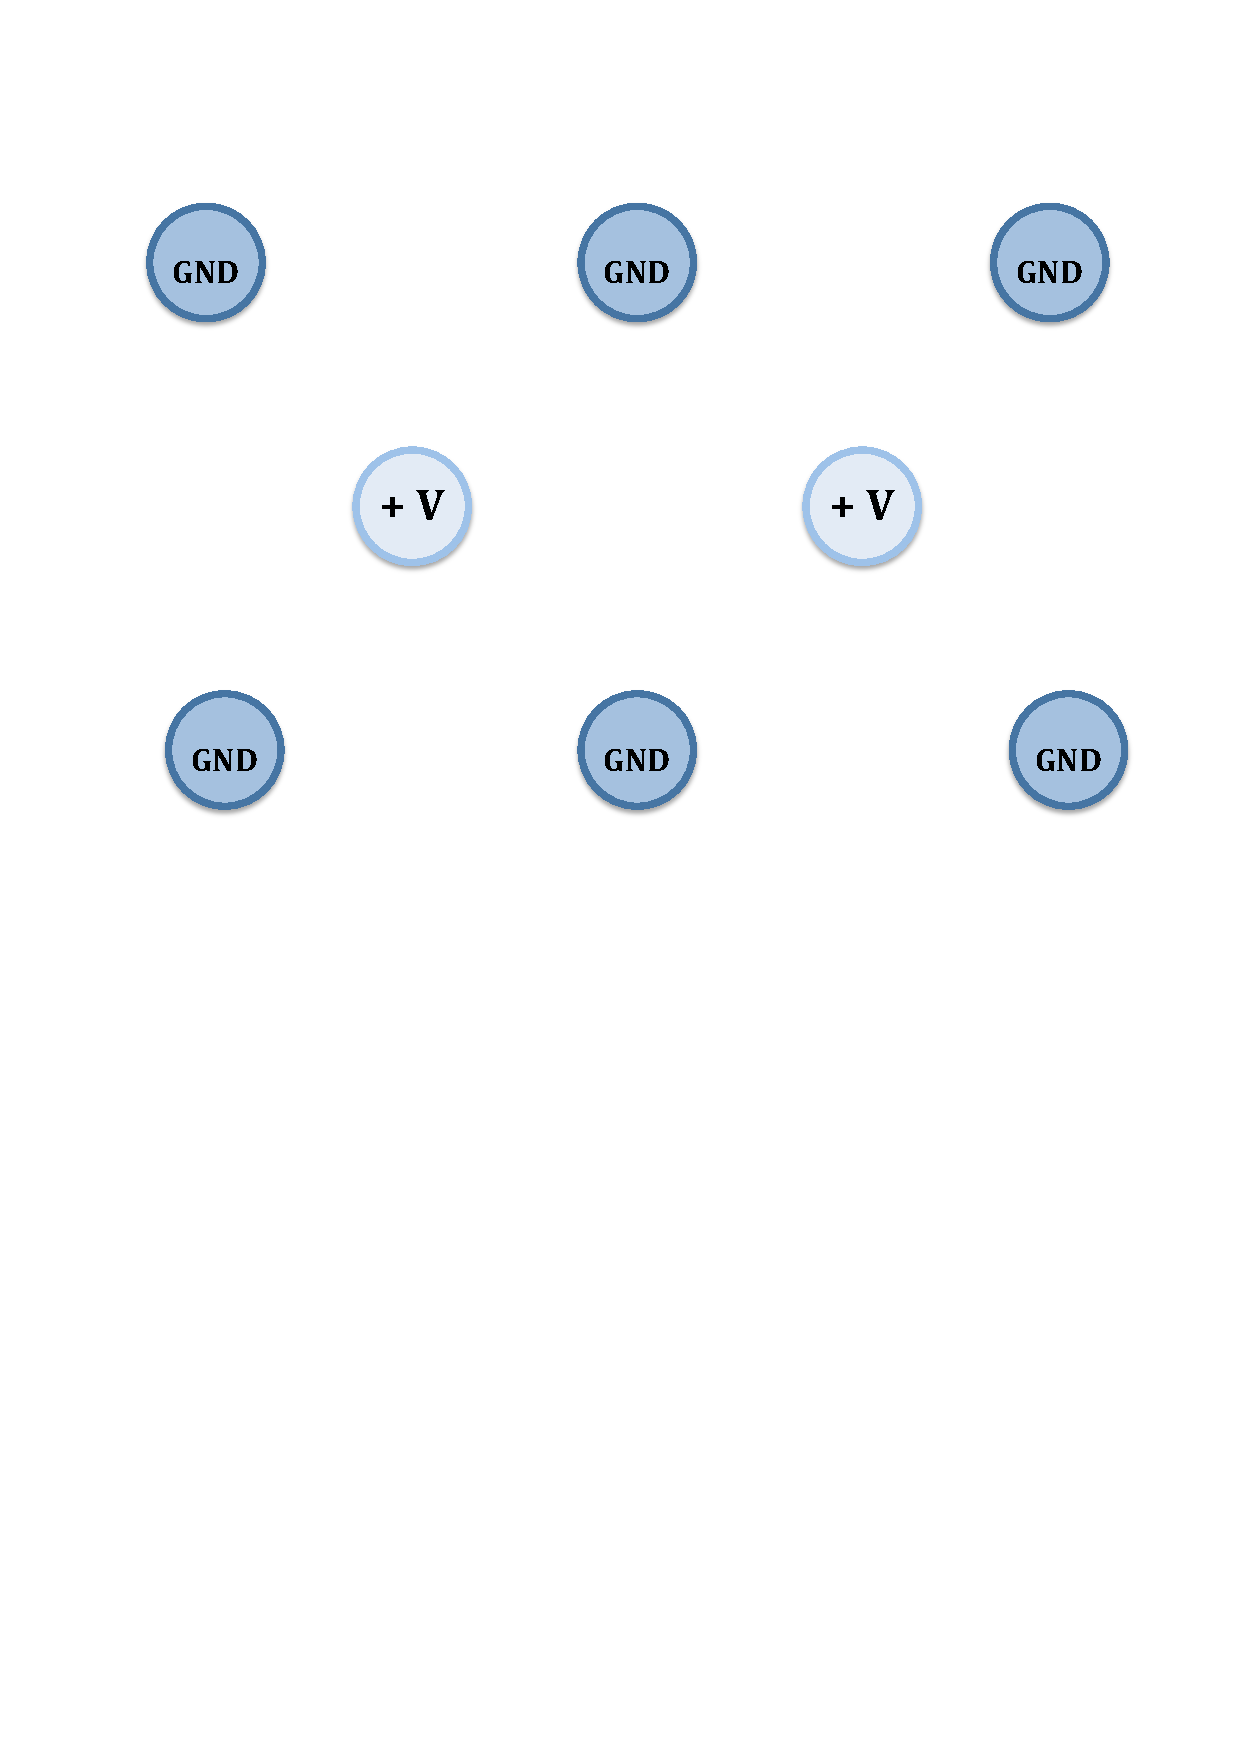
\includegraphics[width=.5\linewidth]{GPdiagramE}
  \captionof{figure}{System E}
  \label{fig:test2}
\end{minipage}
\end{figure}
%[width=.4\linewidth] %add after includegraphs

\end{document}
